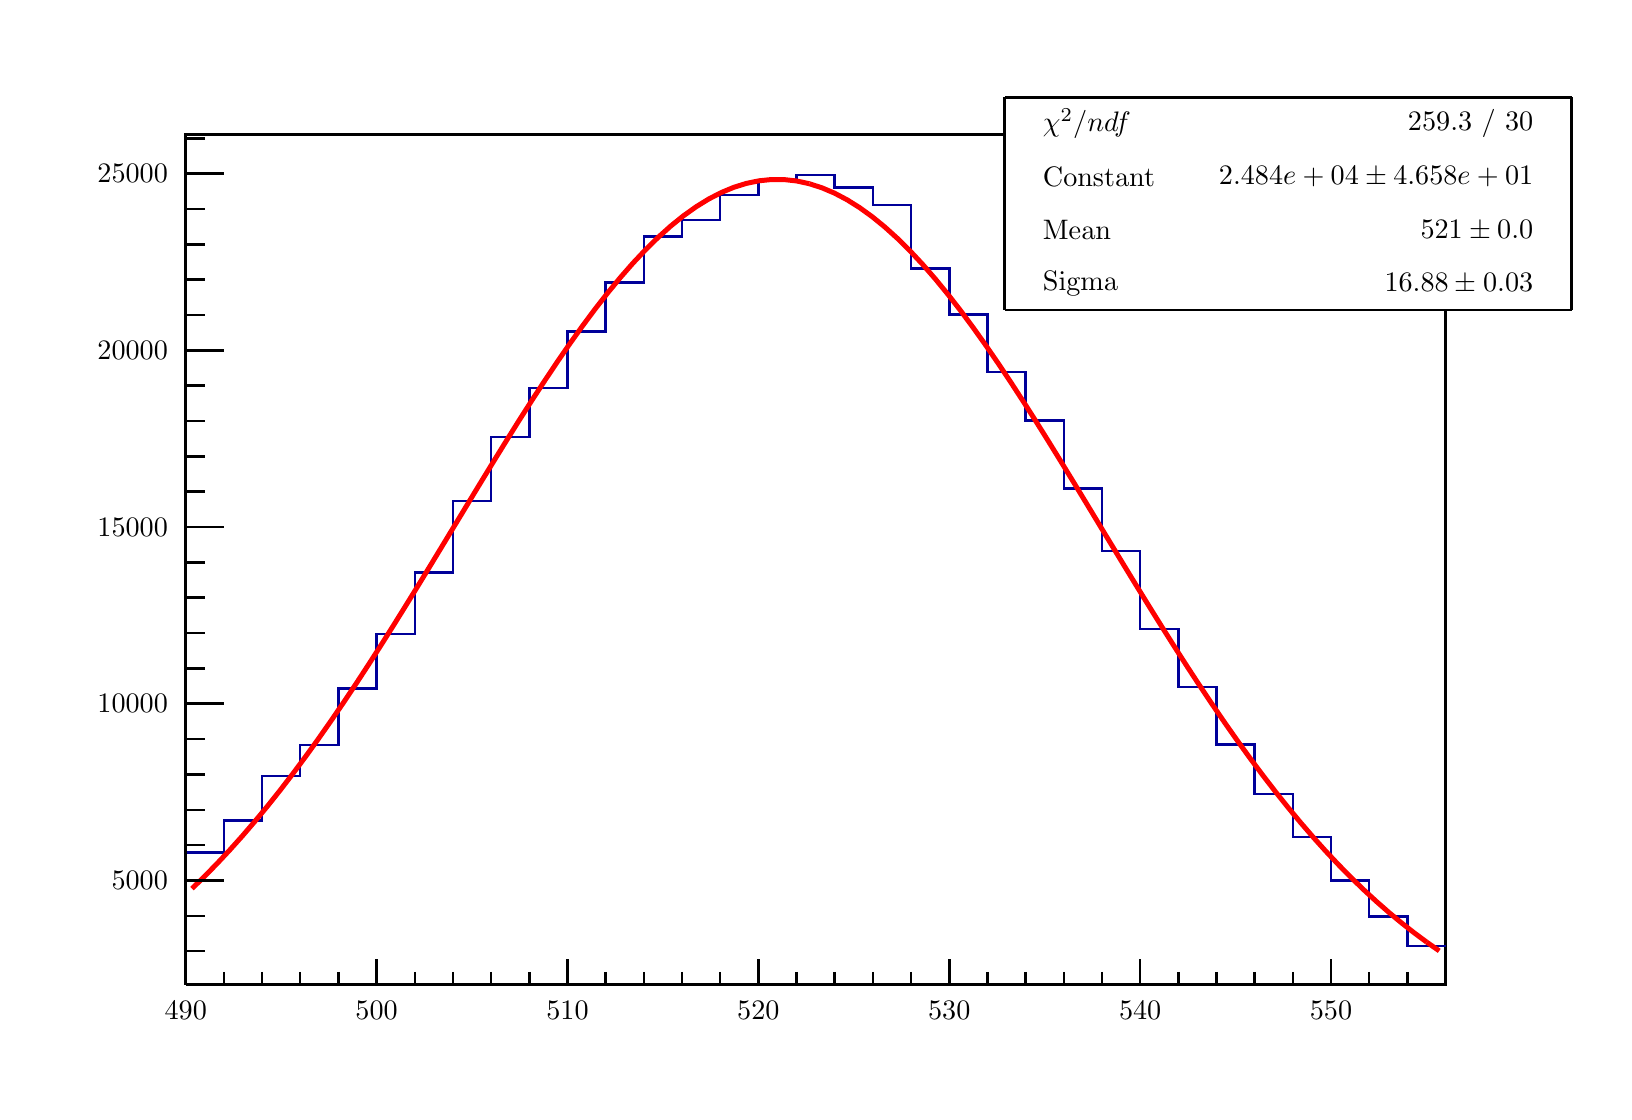
\begin{tikzpicture}
\pgfdeclareplotmark{cross} {
\pgfpathmoveto{\pgfpoint{-0.3\pgfplotmarksize}{\pgfplotmarksize}}
\pgfpathlineto{\pgfpoint{+0.3\pgfplotmarksize}{\pgfplotmarksize}}
\pgfpathlineto{\pgfpoint{+0.3\pgfplotmarksize}{0.3\pgfplotmarksize}}
\pgfpathlineto{\pgfpoint{+1\pgfplotmarksize}{0.3\pgfplotmarksize}}
\pgfpathlineto{\pgfpoint{+1\pgfplotmarksize}{-0.3\pgfplotmarksize}}
\pgfpathlineto{\pgfpoint{+0.3\pgfplotmarksize}{-0.3\pgfplotmarksize}}
\pgfpathlineto{\pgfpoint{+0.3\pgfplotmarksize}{-1.\pgfplotmarksize}}
\pgfpathlineto{\pgfpoint{-0.3\pgfplotmarksize}{-1.\pgfplotmarksize}}
\pgfpathlineto{\pgfpoint{-0.3\pgfplotmarksize}{-0.3\pgfplotmarksize}}
\pgfpathlineto{\pgfpoint{-1.\pgfplotmarksize}{-0.3\pgfplotmarksize}}
\pgfpathlineto{\pgfpoint{-1.\pgfplotmarksize}{0.3\pgfplotmarksize}}
\pgfpathlineto{\pgfpoint{-0.3\pgfplotmarksize}{0.3\pgfplotmarksize}}
\pgfpathclose
\pgfusepathqstroke
}
\pgfdeclareplotmark{cross*} {
\pgfpathmoveto{\pgfpoint{-0.3\pgfplotmarksize}{\pgfplotmarksize}}
\pgfpathlineto{\pgfpoint{+0.3\pgfplotmarksize}{\pgfplotmarksize}}
\pgfpathlineto{\pgfpoint{+0.3\pgfplotmarksize}{0.3\pgfplotmarksize}}
\pgfpathlineto{\pgfpoint{+1\pgfplotmarksize}{0.3\pgfplotmarksize}}
\pgfpathlineto{\pgfpoint{+1\pgfplotmarksize}{-0.3\pgfplotmarksize}}
\pgfpathlineto{\pgfpoint{+0.3\pgfplotmarksize}{-0.3\pgfplotmarksize}}
\pgfpathlineto{\pgfpoint{+0.3\pgfplotmarksize}{-1.\pgfplotmarksize}}
\pgfpathlineto{\pgfpoint{-0.3\pgfplotmarksize}{-1.\pgfplotmarksize}}
\pgfpathlineto{\pgfpoint{-0.3\pgfplotmarksize}{-0.3\pgfplotmarksize}}
\pgfpathlineto{\pgfpoint{-1.\pgfplotmarksize}{-0.3\pgfplotmarksize}}
\pgfpathlineto{\pgfpoint{-1.\pgfplotmarksize}{0.3\pgfplotmarksize}}
\pgfpathlineto{\pgfpoint{-0.3\pgfplotmarksize}{0.3\pgfplotmarksize}}
\pgfpathclose
\pgfusepathqfillstroke
}
\pgfdeclareplotmark{newstar} {
\pgfpathmoveto{\pgfqpoint{0pt}{\pgfplotmarksize}}
\pgfpathlineto{\pgfqpointpolar{44}{0.5\pgfplotmarksize}}
\pgfpathlineto{\pgfqpointpolar{18}{\pgfplotmarksize}}
\pgfpathlineto{\pgfqpointpolar{-20}{0.5\pgfplotmarksize}}
\pgfpathlineto{\pgfqpointpolar{-54}{\pgfplotmarksize}}
\pgfpathlineto{\pgfqpointpolar{-90}{0.5\pgfplotmarksize}}
\pgfpathlineto{\pgfqpointpolar{234}{\pgfplotmarksize}}
\pgfpathlineto{\pgfqpointpolar{198}{0.5\pgfplotmarksize}}
\pgfpathlineto{\pgfqpointpolar{162}{\pgfplotmarksize}}
\pgfpathlineto{\pgfqpointpolar{134}{0.5\pgfplotmarksize}}
\pgfpathclose
\pgfusepathqstroke
}
\pgfdeclareplotmark{newstar*} {
\pgfpathmoveto{\pgfqpoint{0pt}{\pgfplotmarksize}}
\pgfpathlineto{\pgfqpointpolar{44}{0.5\pgfplotmarksize}}
\pgfpathlineto{\pgfqpointpolar{18}{\pgfplotmarksize}}
\pgfpathlineto{\pgfqpointpolar{-20}{0.5\pgfplotmarksize}}
\pgfpathlineto{\pgfqpointpolar{-54}{\pgfplotmarksize}}
\pgfpathlineto{\pgfqpointpolar{-90}{0.5\pgfplotmarksize}}
\pgfpathlineto{\pgfqpointpolar{234}{\pgfplotmarksize}}
\pgfpathlineto{\pgfqpointpolar{198}{0.5\pgfplotmarksize}}
\pgfpathlineto{\pgfqpointpolar{162}{\pgfplotmarksize}}
\pgfpathlineto{\pgfqpointpolar{134}{0.5\pgfplotmarksize}}
\pgfpathclose
\pgfusepathqfillstroke
}
\definecolor{c}{rgb}{1,1,1};
\draw [color=c, fill=c] (0,0) rectangle (20,13.4957);
\draw [color=c, fill=c] (2,1.34957) rectangle (18,12.1461);
\definecolor{c}{rgb}{0,0,0};
\draw [c,line width=0.9] (2,1.34957) -- (2,12.1461) -- (18,12.1461) -- (18,1.34957) -- (2,1.34957);
\definecolor{c}{rgb}{1,1,1};
\draw [color=c, fill=c] (2,1.34957) rectangle (18,12.1461);
\definecolor{c}{rgb}{0,0,0};
\draw [c,line width=0.9] (2,1.34957) -- (2,12.1461) -- (18,12.1461) -- (18,1.34957) -- (2,1.34957);
\definecolor{c}{rgb}{0,0,0.6};
\draw [c,line width=0.9] (2,3.02763) -- (2.48485,3.02763) -- (2.48485,3.432) -- (2.9697,3.432) -- (2.9697,3.99883) -- (3.45455,3.99883) -- (3.45455,4.39243) -- (3.93939,4.39243) -- (3.93939,5.10916) -- (4.42424,5.10916) -- (4.42424,5.80211) --
 (4.90909,5.80211) -- (4.90909,6.58436) -- (5.39394,6.58436) -- (5.39394,7.49184) -- (5.87879,7.49184) -- (5.87879,8.30596) -- (6.36364,8.30596) -- (6.36364,8.92799) -- (6.84848,8.92799) -- (6.84848,9.64697) -- (7.33333,9.64697) -- (7.33333,10.2641)
 -- (7.81818,10.2641) -- (7.81818,10.8515) -- (8.30303,10.8515) -- (8.30303,11.0607) -- (8.78788,11.0607) -- (8.78788,11.3748) -- (9.27273,11.3748) -- (9.27273,11.5674) -- (9.75758,11.5674) -- (9.75758,11.632) -- (10.2424,11.632) -- (10.2424,11.4731)
 -- (10.7273,11.4731) -- (10.7273,11.2537) -- (11.2121,11.2537) -- (11.2121,10.4449) -- (11.697,10.4449) -- (11.697,9.85791) -- (12.1818,9.85791) -- (12.1818,9.12906) -- (12.6667,9.12906) -- (12.6667,8.51375) -- (13.1515,8.51375) -- (13.1515,7.65296)
 -- (13.6364,7.65296) -- (13.6364,6.85454) -- (14.1212,6.85454) -- (14.1212,5.86808) -- (14.6061,5.86808) -- (14.6061,5.1316) -- (15.0909,5.1316) -- (15.0909,4.4014) -- (15.5758,4.4014) -- (15.5758,3.77129) -- (16.0606,3.77129) -- (16.0606,3.22151)
 -- (16.5455,3.22151) -- (16.5455,2.67218) -- (17.0303,2.67218) -- (17.0303,2.21306) -- (17.5152,2.21306) -- (17.5152,1.83921) -- (18,1.83921);
\definecolor{c}{rgb}{1,0,0};
\draw [c,line width=1.8] (2.08,2.56914) -- (2.24,2.72499) -- (2.4,2.88843) -- (2.56,3.05947) -- (2.72,3.2381) -- (2.88,3.42428) -- (3.04,3.61792) -- (3.2,3.81888) -- (3.36,4.027) -- (3.52,4.24205) -- (3.68,4.46379) -- (3.84,4.69188) -- (4,4.92599) --
 (4.16,5.16571) -- (4.32,5.41057) -- (4.48,5.66009) -- (4.64,5.91371) -- (4.8,6.17083) -- (4.96,6.43082) -- (5.12,6.69299) -- (5.28,6.95662) -- (5.44,7.22094) -- (5.6,7.48517) -- (5.76,7.74848) -- (5.92,8.01) -- (6.08,8.26887) -- (6.24,8.52419) --
 (6.4,8.77504) -- (6.56,9.02052) -- (6.72,9.2597) -- (6.88,9.49166) -- (7.04,9.7155) -- (7.2,9.93033) -- (7.36,10.1353) -- (7.52,10.3295) -- (7.68,10.5121) -- (7.84,10.6825) -- (8,10.8397) -- (8.16,10.9833) -- (8.32,11.1124) -- (8.48,11.2266) --
 (8.64,11.3254) -- (8.8,11.4082) -- (8.96,11.4748) -- (9.12,11.5248) -- (9.28,11.5579) -- (9.44,11.5742) -- (9.6,11.5733) -- (9.76,11.5555) -- (9.92,11.5207);
\draw [c,line width=1.8] (9.92,11.5207) -- (10.08,11.4691) -- (10.24,11.401) -- (10.4,11.3166) -- (10.56,11.2163) -- (10.72,11.1006) -- (10.88,10.9701) -- (11.04,10.8252) -- (11.2,10.6667) -- (11.36,10.4951) -- (11.52,10.3113) -- (11.68,10.116) --
 (11.84,9.91011) -- (12,9.69438) -- (12.16,9.46972) -- (12.32,9.23702) -- (12.48,8.9972) -- (12.64,8.75117) -- (12.8,8.49984) -- (12.96,8.24415) -- (13.12,7.98498) -- (13.28,7.72325) -- (13.44,7.45982) -- (13.6,7.19555) -- (13.76,6.93125) --
 (13.92,6.66773) -- (14.08,6.40574) -- (14.24,6.146) -- (14.4,5.88918) -- (14.56,5.63594) -- (14.72,5.38684) -- (14.88,5.14245) -- (15.04,4.90326) -- (15.2,4.66971) -- (15.36,4.44221) -- (15.52,4.2211) -- (15.68,4.0067) -- (15.84,3.79926) --
 (16,3.599) -- (16.16,3.40608) -- (16.32,3.22062) -- (16.48,3.04271) -- (16.64,2.8724) -- (16.8,2.70969) -- (16.96,2.55456) -- (17.12,2.40696) -- (17.28,2.26679) -- (17.44,2.13394) -- (17.6,2.00827) -- (17.76,1.88963);
\draw [c,line width=1.8] (17.76,1.88963) -- (17.92,1.77783);
\definecolor{c}{rgb}{1,1,1};
\draw [color=c, fill=c] (12.4,9.91934) rectangle (19.6,12.6185);
\definecolor{c}{rgb}{0,0,0};
\draw [c,line width=0.9] (12.4,9.91934) -- (19.6,9.91934);
\draw [c,line width=0.9] (19.6,9.91934) -- (19.6,12.6185);
\draw [c,line width=0.9] (19.6,12.6185) -- (12.4,12.6185);
\draw [c,line width=0.9] (12.4,12.6185) -- (12.4,9.91934);
\draw [anchor= west] (12.76,12.2811) node[scale=1.01821, color=c, rotate=0]{$\chi^{2} / ndf $};
\draw [anchor= east] (19.24,12.2811) node[scale=1.01821, color=c, rotate=0]{ 259.3 / 30};
\draw [anchor= west] (12.76,11.6063) node[scale=1.01821, color=c, rotate=0]{Constant };
\draw [anchor= east] (19.24,11.6063) node[scale=1.01821, color=c, rotate=0]{$ 2.484e+04 \pm 4.658e+01$};
\draw [anchor= west] (12.76,10.9315) node[scale=1.01821, color=c, rotate=0]{Mean     };
\draw [anchor= east] (19.24,10.9315) node[scale=1.01821, color=c, rotate=0]{$   521 \pm 0.0$};
\draw [anchor= west] (12.76,10.2567) node[scale=1.01821, color=c, rotate=0]{Sigma    };
\draw [anchor= east] (19.24,10.2567) node[scale=1.01821, color=c, rotate=0]{$ 16.88 \pm 0.03$};
\draw [c,line width=0.9] (2,1.34957) -- (18,1.34957);
\draw [c,line width=0.9] (2,1.67347) -- (2,1.34957);
\draw [c,line width=0.9] (2.48485,1.51152) -- (2.48485,1.34957);
\draw [c,line width=0.9] (2.9697,1.51152) -- (2.9697,1.34957);
\draw [c,line width=0.9] (3.45455,1.51152) -- (3.45455,1.34957);
\draw [c,line width=0.9] (3.93939,1.51152) -- (3.93939,1.34957);
\draw [c,line width=0.9] (4.42424,1.67347) -- (4.42424,1.34957);
\draw [c,line width=0.9] (4.90909,1.51152) -- (4.90909,1.34957);
\draw [c,line width=0.9] (5.39394,1.51152) -- (5.39394,1.34957);
\draw [c,line width=0.9] (5.87879,1.51152) -- (5.87879,1.34957);
\draw [c,line width=0.9] (6.36364,1.51152) -- (6.36364,1.34957);
\draw [c,line width=0.9] (6.84848,1.67347) -- (6.84848,1.34957);
\draw [c,line width=0.9] (7.33333,1.51152) -- (7.33333,1.34957);
\draw [c,line width=0.9] (7.81818,1.51152) -- (7.81818,1.34957);
\draw [c,line width=0.9] (8.30303,1.51152) -- (8.30303,1.34957);
\draw [c,line width=0.9] (8.78788,1.51152) -- (8.78788,1.34957);
\draw [c,line width=0.9] (9.27273,1.67347) -- (9.27273,1.34957);
\draw [c,line width=0.9] (9.75758,1.51152) -- (9.75758,1.34957);
\draw [c,line width=0.9] (10.2424,1.51152) -- (10.2424,1.34957);
\draw [c,line width=0.9] (10.7273,1.51152) -- (10.7273,1.34957);
\draw [c,line width=0.9] (11.2121,1.51152) -- (11.2121,1.34957);
\draw [c,line width=0.9] (11.697,1.67347) -- (11.697,1.34957);
\draw [c,line width=0.9] (12.1818,1.51152) -- (12.1818,1.34957);
\draw [c,line width=0.9] (12.6667,1.51152) -- (12.6667,1.34957);
\draw [c,line width=0.9] (13.1515,1.51152) -- (13.1515,1.34957);
\draw [c,line width=0.9] (13.6364,1.51152) -- (13.6364,1.34957);
\draw [c,line width=0.9] (14.1212,1.67347) -- (14.1212,1.34957);
\draw [c,line width=0.9] (14.6061,1.51152) -- (14.6061,1.34957);
\draw [c,line width=0.9] (15.0909,1.51152) -- (15.0909,1.34957);
\draw [c,line width=0.9] (15.5758,1.51152) -- (15.5758,1.34957);
\draw [c,line width=0.9] (16.0606,1.51152) -- (16.0606,1.34957);
\draw [c,line width=0.9] (16.5455,1.67347) -- (16.5455,1.34957);
\draw [c,line width=0.9] (16.5455,1.67347) -- (16.5455,1.34957);
\draw [c,line width=0.9] (17.0303,1.51152) -- (17.0303,1.34957);
\draw [c,line width=0.9] (17.5152,1.51152) -- (17.5152,1.34957);
\draw [c,line width=0.9] (18,1.51152) -- (18,1.34957);
\draw [anchor=base] (2,0.904212) node[scale=1.01821, color=c, rotate=0]{490};
\draw [anchor=base] (4.42424,0.904212) node[scale=1.01821, color=c, rotate=0]{500};
\draw [anchor=base] (6.84848,0.904212) node[scale=1.01821, color=c, rotate=0]{510};
\draw [anchor=base] (9.27273,0.904212) node[scale=1.01821, color=c, rotate=0]{520};
\draw [anchor=base] (11.697,0.904212) node[scale=1.01821, color=c, rotate=0]{530};
\draw [anchor=base] (14.1212,0.904212) node[scale=1.01821, color=c, rotate=0]{540};
\draw [anchor=base] (16.5455,0.904212) node[scale=1.01821, color=c, rotate=0]{550};
\draw [c,line width=0.9] (2,1.34957) -- (2,12.1461);
\draw [c,line width=0.9] (2.48,2.67263) -- (2,2.67263);
\draw [c,line width=0.9] (2.24,3.12143) -- (2,3.12143);
\draw [c,line width=0.9] (2.24,3.57023) -- (2,3.57023);
\draw [c,line width=0.9] (2.24,4.01903) -- (2,4.01903);
\draw [c,line width=0.9] (2.24,4.46783) -- (2,4.46783);
\draw [c,line width=0.9] (2.48,4.91663) -- (2,4.91663);
\draw [c,line width=0.9] (2.24,5.36543) -- (2,5.36543);
\draw [c,line width=0.9] (2.24,5.81423) -- (2,5.81423);
\draw [c,line width=0.9] (2.24,6.26302) -- (2,6.26302);
\draw [c,line width=0.9] (2.24,6.71182) -- (2,6.71182);
\draw [c,line width=0.9] (2.48,7.16062) -- (2,7.16062);
\draw [c,line width=0.9] (2.24,7.60942) -- (2,7.60942);
\draw [c,line width=0.9] (2.24,8.05822) -- (2,8.05822);
\draw [c,line width=0.9] (2.24,8.50702) -- (2,8.50702);
\draw [c,line width=0.9] (2.24,8.95582) -- (2,8.95582);
\draw [c,line width=0.9] (2.48,9.40462) -- (2,9.40462);
\draw [c,line width=0.9] (2.24,9.85342) -- (2,9.85342);
\draw [c,line width=0.9] (2.24,10.3022) -- (2,10.3022);
\draw [c,line width=0.9] (2.24,10.751) -- (2,10.751);
\draw [c,line width=0.9] (2.24,11.1998) -- (2,11.1998);
\draw [c,line width=0.9] (2.48,11.6486) -- (2,11.6486);
\draw [c,line width=0.9] (2.48,2.67263) -- (2,2.67263);
\draw [c,line width=0.9] (2.24,2.22383) -- (2,2.22383);
\draw [c,line width=0.9] (2.24,1.77503) -- (2,1.77503);
\draw [c,line width=0.9] (2.48,11.6486) -- (2,11.6486);
\draw [c,line width=0.9] (2.24,12.0974) -- (2,12.0974);
\draw [anchor= east] (1.9,2.67263) node[scale=1.01821, color=c, rotate=0]{5000};
\draw [anchor= east] (1.9,4.91663) node[scale=1.01821, color=c, rotate=0]{10000};
\draw [anchor= east] (1.9,7.16062) node[scale=1.01821, color=c, rotate=0]{15000};
\draw [anchor= east] (1.9,9.40462) node[scale=1.01821, color=c, rotate=0]{20000};
\draw [anchor= east] (1.9,11.6486) node[scale=1.01821, color=c, rotate=0]{25000};
\definecolor{c}{rgb}{1,1,1};
\draw [color=c, fill=c] (12.4,9.91934) rectangle (19.6,12.6185);
\definecolor{c}{rgb}{0,0,0};
\draw [c,line width=0.9] (12.4,9.91934) -- (19.6,9.91934);
\draw [c,line width=0.9] (19.6,9.91934) -- (19.6,12.6185);
\draw [c,line width=0.9] (19.6,12.6185) -- (12.4,12.6185);
\draw [c,line width=0.9] (12.4,12.6185) -- (12.4,9.91934);
\draw [anchor= west] (12.76,12.2811) node[scale=1.01821, color=c, rotate=0]{$\chi^{2} / ndf $};
\draw [anchor= east] (19.24,12.2811) node[scale=1.01821, color=c, rotate=0]{ 259.3 / 30};
\draw [anchor= west] (12.76,11.6063) node[scale=1.01821, color=c, rotate=0]{Constant };
\draw [anchor= east] (19.24,11.6063) node[scale=1.01821, color=c, rotate=0]{$ 2.484e+04 \pm 4.658e+01$};
\draw [anchor= west] (12.76,10.9315) node[scale=1.01821, color=c, rotate=0]{Mean     };
\draw [anchor= east] (19.24,10.9315) node[scale=1.01821, color=c, rotate=0]{$   521 \pm 0.0$};
\draw [anchor= west] (12.76,10.2567) node[scale=1.01821, color=c, rotate=0]{Sigma    };
\draw [anchor= east] (19.24,10.2567) node[scale=1.01821, color=c, rotate=0]{$ 16.88 \pm 0.03$};
\end{tikzpicture}
